\documentclass[a4paper,12pt,titlepage]{scrartcl}
\usepackage[T1]{fontenc}
\usepackage[utf8]{inputenc}
\usepackage[ngerman]{babel}
\usepackage{graphicx}                         
\usepackage{float}
\usepackage{hyperref}
\usepackage{listings}
\usepackage{tikz}
\usetikzlibrary{automata,arrows,positioning,fit,shapes,calc}

\usepackage{fancyhdr}
\renewcommand{\headrulewidth}{0.5pt}
\renewcommand{\footrulewidth}{0.5pt}
%Abstand zwischen Absätzen, Zeilenabstände
\voffset26pt 
\parskip6pt
%\parindent1cm  %Rückt erste Zeile eines neuen Absatzes ein
\usepackage{setspace}
\onehalfspacing

\begin{document}
\pagenumbering{roman}
\titlehead
{
    \small
    {
        Technische Universität Ilmenau\\
        Fakulät IA\\
        Fachgebiet Schaltsysteme\\

        Praktikum Schaltsysteme\\
        WS 2021/22}
}

\title {Versuchsprotokoll}
\subtitle{Versuche A2, A3, A4 und A10}
\author{}
\date{09.12.2021\\*[60pt]}
\maketitle

\pagestyle{fancy}
\fancyhead[R]{Praktikumsbericht: Schaltsysteme}
\pagenumbering{arabic}
\newpage

\section*{Aufgabe 2: Rechts/Links-Impulserzeugung}
\subsection*{Aufgabenstellung}
Entwerfen Sie einen Automaten zur Ermittlung der relativen x-Position einer PC-Maus.
Das Maus-Modul generiert die Signale $x_0$ und $x_1$ entsprechend der folgenden Kurvenverläufe.
Durch den Automaten sind entsprechend dem angegebenen Impulsschema die Signale $l$ und $r$ zu generieren, die zur Anzeige der relativen Position an einen Vor-/Rückwärtszähler angeschlossen werden sollen.

\begin{center}
    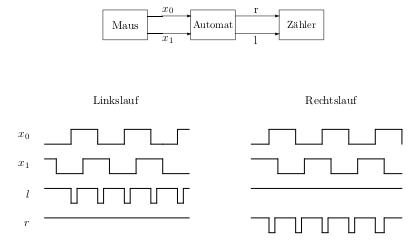
\includegraphics[width=.5\linewidth]{Assets/Schaltsysteme-praktika-v2.png}
\end{center}

\subsection*{Lösungsweg und Entwicklung der Blockstruktur}
Beim Linkslauf folgt der $x_1$ Pegel auf den $x_0$ Pegel und der Ausgang $l$ wird bei jeder Flanke von $x_0$ auf Null gesetzt (und kurz darauf wieder zurück).

Beim Rechtslauf folgt der $x_0$ Pegel auf den $x_1$ Pegel und der Ausgang $r$ wird bei jeder Flanke von $x_1$ auf Null gesetzt (und kurz darauf wieder zurück).

Das Signal $x_0$ wird als Takt verwendet und das Signal $x_1$ für die Rechts-Links-Entscheidung.
Es wird zwischen drei Zuständen $z_0,z_1$ und $z_3$ unterschieden.

\subsection*{Ermittlung der Funktion der sequentiellen Automaten}
\begin{center}
    \begin{tikzpicture}[node distance=5cm,
            ->, % makes the edges directed
            every state/.style={thick, fill=gray!10}, % sets the properties for each ’state’ node
        ]
        \node[state] (z0) {$z_0$ \nodepart{lower} $l=1;r=1$};
        \node[state, left of=z0] (z1) {$z_1$ \nodepart{lower} $l=0;r=1$};
        \node[state, right of=z0] (z2) {$z_2$ \nodepart{lower} $l=1;r=0$};
        \draw
        (z0) edge[bend right, above] node{$x_0\overline{x_1} \vee \overline{x_0} x_1$} (z1)
        (z1) edge[bend right, below] node{$x_0\vee x_1$} (z0)

        (z0) edge[bend right, below] node{$\overline{x_0x_1} \vee x_0 x_1$} (z2)
        (z2) edge[bend right, above] node{$x_0\vee x_1$} (z0);
        ;
    \end{tikzpicture}
\end{center}
\newpage

\section*{Aufgabe 3: Kreuztisch}
\subsection*{Aufgabenstellung}
Gesucht ist ein Steuerwerk, welches durch Auswertung der Positionssignale $x_l,x_r,x_u,x_o$ und Erzeugung der Motorsteuersignale $y_l,y_r,y_u,y_o$ folgenden Ablauf realisiert:
\begin{itemize}
    \item Der Punkt P soll unabhängig von seiner Anfangsstellung nach der Pulldown-Flanke von $x_s$ möglichst schnell nach links/unten bewegt werden.
    \item Danach soll er am linken Rand nach oben
    \item und am oberen Rand nach rechts gefahren werden, worauf die Bewegung gestoppt werden soll.
\end{itemize}
Ein Neustart ist nur mit einer erneuten Pulldown-Flanke von $x_s$ möglich.

\begin{center}
    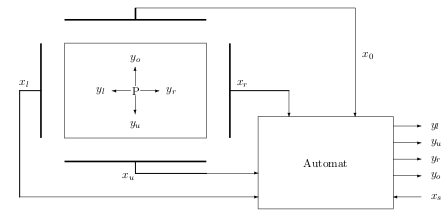
\includegraphics[width=.6\linewidth]{Assets/Schaltsysteme-praktika-v3.png}
\end{center}

\subsection*{Lösungsweg und Entwicklung der Blockstruktur}
...
\subsection*{Ermittlung der Funktion der sequentiellen Automaten}
...
\subsection*{Synthese der Schaltungsstruktur}
...
\newpage

\section*{Aufgabe 4: Pumpensteuerung (statisch)}
\subsection*{Aufgabenstellung}
Entsprechend der folgenden Skizze sollen zwei Pumpen einen Wasserbehälter füllen. Das Verhalten der Verbraucher ist nicht bekannt.
Die vier Füllstandsmelder $x_0$ bis $x_3$ sprechen jeweils bei Überschreitung eines bestimmten Füllstandes statisch an.
Die Pumpen sollen entsprechend dem angegebenen Diagramm arbeiten, wobei die Schalthäufigkeit der Pumpen gleich verteilt sein soll. Um ein ,,Flattern'' der Pumpen bei Füllständen im Bereich der jeweiligen Füllstandsmelder zu vermeiden, ist das gegebene Hystereseverhalten zu realisieren.
Entwerfen Sie eine Steuerung, die diese Aufgabe realisiert!

\begin{center}
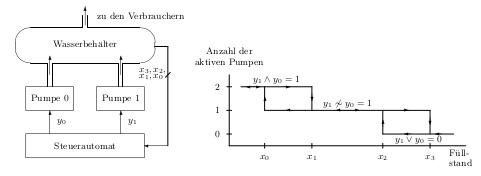
\includegraphics[width=.5\linewidth]{Assets/Schaltsysteme-praktika-v4.png}
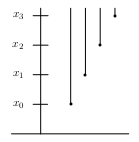
\includegraphics[width=.15\linewidth]{Assets/Schaltsysteme-praktika-v4-2.png}
\end{center}

Hinweis: Bei Erreichen eines Schaltpunktes wird das Signal statisch auf 1 gesetzt. Alle Füllstandsmelder, die vom Wasser bedeckt sind, bleiben gesetzt, d.h. für den obersten Schaltpunkt ergibt sich: $x_3 x_2 x_1 x_0$.

\subsection*{Lösungsweg und Entwicklung der Blockstruktur}
Wie nehmen der Einfachheit halber an, der Behälter anfangs vollständig mit Wasser gefüllt ist. Das System könnte aber auch in jedem anderen Zustand starten. In diesem Zustand sind beide Pumpen aus, denn der Wasserspiegel befindet sich über dem Soll-Wasserspiegel. Also pumpen die Pumpen kein zusätzliches Wasser dazu und der Wasserspiegel sinkt. Solange Sensor $x_2$ noch mit Wasser bedeckt ist, ändert sich nichts. Sobald aber das Wasser unter $x_2$ sinkt, springt die erste Pumpe an und pumpt Wasser in den Behälter. Sinkt das Wasser dann noch weiter, bis Sensor $x_0$ auch nicht mehr vom Wasser bedeckt wird, dann schaltet sich auch die zweite Pumpe ein. Nun laufen beide Pumpen solange bis der Wasserspiegel wieder über $x_1$ steigt. Dann schaltet sich eine Pumpe ab und es läuft wieder nur eine Pumpe. Hierbei ist wichtig, dass nun die andere Pumpe läuft, als die die als letztes allein lief. Die Kodierung der Zustände geschieht in der Reihenfolge $z_2,z_1,z_0$.

\subsection*{Ermittlung der Funktion der sequentiellen Automaten}
\begin{center}
    \begin{tikzpicture}[node distance=4cm,
            ->, % makes the edges directed
            every state/.style={thick, fill=gray!10}, % sets the properties for each ’state’ node
        ]
        \node (000) [state with output]                 {000 \nodepart{lower} $y_0=0;y_1=0$};
        \node (001) [state with output, right of=000]   {001 \nodepart{lower} $y_0=1;y_1=0$};
        \node (010) [state with output, right of=001]   {010 \nodepart{lower} $y_0=1;y_1=1$};
        \node (100) [state with output, below of=000]   {100 \nodepart{lower} $y_0=0;y_1=0$};
        \node (101) [state with output, right of=100]   {101 \nodepart{lower} $y_0=0;y_1=1$};
        \node (111) [state with output, right of=101]   {111 \nodepart{lower} $y_0=1;y_1=1$};

        \draw
        (000) edge[loop above] node{$x_2$} (000)
        (000) edge[above] node{$\overline{x_2}$} (001)

        (001) edge[loop above] node{$\overline{x_3}x_0$} (001)
        (001) edge[above] node{$\overline{x_0}$} (010)
        (001) edge[above] node{$x_3$} (100)

        (010) edge[loop above] node{$\overline{x_1}$} (010)
        (010) edge[above] node{$x_1$} (101)

        (100) edge[loop below] node{$x_2$} (100)
        (100) edge[above] node{$\overline{x_2}$} (101)

        (101) edge[loop below] node{$\overline{x_3}x_0$} (101)
        (101) edge[above] node{$\overline{x_0}$} (111)
        (101) edge[above] node{$x_3$} (000)

        (111) edge[loop below] node{$\overline{x_1}$} (111)
        (111) edge[above] node{$x_1$} (001);
    \end{tikzpicture}
\end{center}

$z_2= z_2\overline{z_1z_0}x_2 \vee \overline{z_2z_1}z_0x_3 \vee z_2\overline{z_1z_0x_2} \vee \overline{z_2}z_1\overline{z_0}x_1 \vee z_2\overline{z_1}z_0\overline{x_3}x_0 \vee z_2\overline{z_1}z_0\overline{x_0} \vee z_2z_1z_0\overline{x_1}$

$z_1=\overline{z_2z_1}z_0\overline{x_0}\vee \overline{z_2}z_1\overline{z_0x_1} \vee z_2z_1z_0\overline{x_1} \vee z_2\overline{z_1}z_0\overline{x_0}$

$z_0=\overline{z_2z_1z_0x_2}\vee z_2z_1z_0x_1 \vee z_2\overline{z_1z_0x_2} \vee z_2\overline{z_1}z_0\overline{x_3}x_0 \vee \overline{z_2}z_1\overline{z_0}x_1\vee z_2\overline{z_1}z_0\overline{x_0} \vee z_2z_1z_0\overline{x_1} \vee \overline{z_2z_1}z_0\overline{x_3}x_0$

$y_1= z_2\overline{z_1}z_0 \vee \overline{z_2}z_1\overline{z_0} \vee z_2z_1z_0$

$y_0= \overline{z_2z_1}z_0\vee \overline{z_2}z_1\overline{z_0}\vee z_2z_1z_0$
\newpage

\subsection*{Synthese der Schaltungsstruktur}
\textbf{*.dcb Datei}
\begin{lstlisting}[name=*.dcb-Datei, basicstyle=\tiny]
    *IDENTIFICATION             ! Identifikation der Schaltung
        Pumpensteuerung
        Robert Jeutter
    *X-NAMES                    ! Deklaration der Eingangsvariablen
        x0, x1, x2, x3;
    *Y-NAMES                    ! Deklaration der Ausgangs-, und Zustandsvariablen
        z0, z1, z2, y0, y1;
    *LOCAL                      ! Deklaration der lokalen Variablen        
    *LEVEL                      ! Polaritaetsumschaltung einzelner Variablen
    *BOOLEAN-EQUATIONS          ! Beschreibung mittels BOOLEscher Gleichungen
    z2 := ( /z2 & /z1 & z0 & x3
        + /z2 & z1 & /z0 & x1
        + z2 & /z1 & z0 & /x0
        + z2 & z1 & z0 & /x1
        + z2 & /z1 & /z0
        + z2 & /z1 & /x3 );

    z1 := ( /z2 & z1 & /z0 & /x1
        + z2 & z1 & z0 & /x1
        + /z1 & z0 & /x0 );

    z0 := ( /z2 & z1 & /z0 & x1
        + z2 & /z1 & z0 & /x0
        + /z1 & /z0 & /x2
        + /z1 & z0 & /x3 & x0
        + z2 & z1 & z0
        + z2 & z0 & /x3 );

    y0 = ( /z2 & /z1 & z0
        + /z2 & z1 & /z0
        + z2 & z1 & z0 );

    y1 = ( /z2 & z1 & /z0
        + z2 & z0 );

    *FUNCTION-TABLE             ! Beschreibung mittels Wertetabelle
    *FLOW-TABLE                 ! Beschreibung mittels einer Ablauftabelle
    *SPECIAL-FUNCTIONS          ! Beschreibung von speziellen Logikeigenschaften
    *END                        ! korrekter Abschluss der Datei
    \end{lstlisting}

\par\noindent\rule{\textwidth}{0.4pt}

\textbf{*.ddv-Datei}
\begin{lstlisting}[name=*.ddv-Datei, basicstyle=\tiny]
    *IDENTIFICATION             ! Identifikation der Schaltung, Versionsvermerk, Autor
        Pumpensteuerung
        Robert Jeutter
    *PLD                        ! Auswahl des entsprechenden PLD-Typs (GAL)
        TYPE = GAL16V8;
    *PINS                       ! Zuordnung der Variablen zu den Bauelemente-Pins
        x3  = 2
        x2  = 3;
        x0  = 4;
        x1  = 5;
        y0  = 13;
        y1  = 14;
        z0  = 15;
        z1  = 16;
        z2  = 17;
    *NODES                      ! Zuordnung von Variablen zu internen Knoten des Bauelements
    *SPECIAL-FUNCTIONS          ! Beschreibung von speziellen Logikeigenschaften des Bauelements
    *FUSES                      ! Direktes Programmieren einer Fuse
    *END
    \end{lstlisting}

\subsection*{Versuchsauswertung}
\begin{center}
    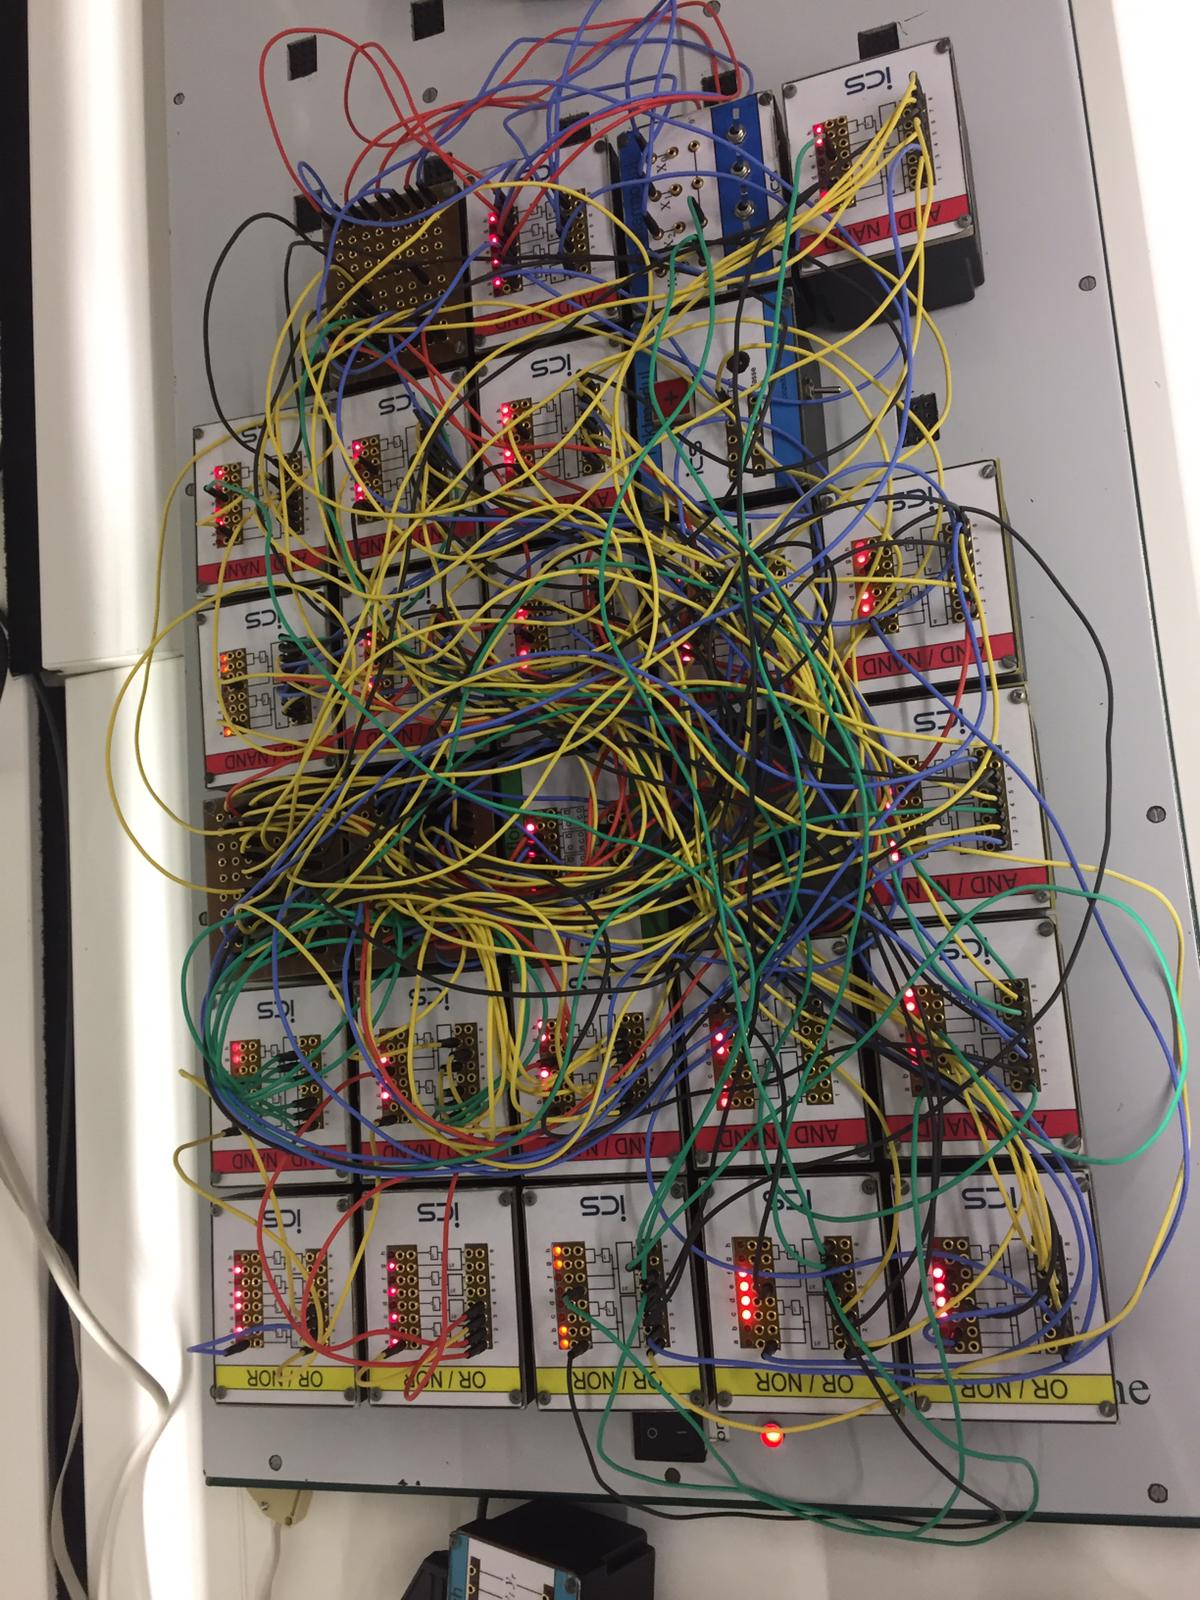
\includegraphics[width=.8\linewidth]{Assets/PraktikumSchaltsysteme.jpeg}
\end{center}

Die fertige Schaltung aus 16 AND- (rot), 5 OR-Gattern (gelb), 1 Taktgeber, 1 Schaltermodul mit 4 Schaltern und 1 D-Flip-Flop. Zur Verteilung der Signale/Anschlüsse wurden zusätzlich 3 Verteiler (Braun) genutzt.

\newpage

\section*{Aufgabe 10: Ampelsteuerung}
\subsection*{Aufgabenstellung}
Es soll eine Ampelsteuerung realisiert werden, die im Ruhezustand für den Autofahrer grün zeigt und auf Anforderung eines Fußgängers diesem das sichere Überqueren der Straße ermöglicht. Die dazu nötigen Phasen zeigt die folgende Tabelle.

\begin{tabular}{c|c|c|c}
    Zustand & Autoampel & Fußgängerampel & Dauer(s)    \\
    S1      & grün      & rot            & Ruhezustand \\
    S2      & gelb      & rot            & 3           \\
    S3      & rot       & rot            & 3           \\
    S4      & rot       & grün           & 24          \\
    S5      & rot       & rot            & 12          \\
    S6      & rot-gelb  & rot            & 3
\end{tabular}

Die Steuerung hat eine Taktfrequenz von $\frac{1}{3}$ Hz.
Entwerfen Sie eine Steuerung, die diese Aufgabe realisiert!

\subsection*{Lösungsweg und Entwicklung der Blockstruktur}
...

\subsection*{Ermittlung der Funktion der sequentiellen Automaten}
...

\subsection*{Synthese der Schaltungsstruktur}
...

\end{document}